\documentclass[final]{thesis} %% Tulostaa tutkielman kuvioiden kanssa!
%\documentclass[draft]{thesis} %% Tulostaa tutkielman ilman kuvioita!

% Tämä tiedostopohja käyttää biblatexia!

%----------------------------------------------------------------------------------------
% PDF-TIEDOSTON INFORMAATIO
%----------------------------------------------------------------------------------------
\hypersetup{%
	pdftitle    = {Title of your report},%
	pdfauthor   = {Onni Opiskelija},%
	pdfsubject  = {Research training (FYSS9470) report},%
	pdfproducer = {pdfTeX}
}

%----------------------------------------------------------------------------------------
% LÄHDELUETTELON MUOTOILU BibLaTeXin käytettäessä
%----------------------------------------------------------------------------------------
\usepackage{csquotes}
\usepackage[backend=biber,style=numeric-comp,sorting=none,maxnames=3,minnames=1,giveninits=true]{biblatex}
\DefineBibliographyStrings{finnish}{%
    andothers  = {ym.},%
    references = {Lähteet},%
    mathesis   = {pro gradu~-tutkielma},%
    phdthesis  = {väitöskirja}
}
\addbibresource{mallilahteet.bib}%----------------------------------------------------------------------------------------
% KANSILEHDEN SISÄLTÖ
%----------------------------------------------------------------------------------------

\title{Title of your report}
\author{Olli Opiskelija}
\supervisor{Matti Meikäläinen\\Heikki Heikäläinen (Company)}
\project{Research Training (FYSS9470) report}
\date{20.1.2020}

%----------------------------------------------------------------------------------------
% KÄYTTÖÖN OTETUT MAKROPAKETIT
% (joita ei ole määritelty dokumenttiluokassa.)
%----------------------------------------------------------------------------------------
\usepackage{amsmath}

%----------------------------------------------------------------------------------------
% VARSINAINEN DOKUMENTTI
%----------------------------------------------------------------------------------------
\begin{document}
%----------------------------------------------------------------------------------------
% KANSILEHTI
%----------------------------------------------------------------------------------------
\titleJYFL


%----------------------------------------------------------------------------------------
%	ABSTRACT
%----------------------------------------------------------------------------------------
\section*{Abstract}
\addcontentsline{toc}{section}{Abstract}

% Bibliographic information
\begin{singlespace}
	Opiskelija, Olli\\
	Title of your report \\
	Research training (FYSS9470) report \\
	Department of Physics, University of Jyväskylä, 2020, \pageref{LastPage}~pages.
\end{singlespace}

\bigskip

% Abstract text
\noindent This should be written in English. \lipsum[1]

\bigskip 

% Keywords
\noindent Keywords: Thesis, abstract, writing, instructions

% --------------------------------------------------------------------------
% ESIPUHE
% --------------------------------------------------------------------------
\section*{Preface}
\addcontentsline{toc}{section}{Preface}

Esipuheen teksti tulee tähän. \lipsum[1]

\bigskip

\noindent Jyväskylä January 1, 2020

\bigskip

\noindent Olli Opiskelija

% --------------------------------------------------------------------------
% SISÄLLYS
% --------------------------------------------------------------------------
\tableofcontents

% --------------------------------------------------------------------------
% VARSINAINEN TEKSTIOSA
% --------------------------------------------------------------------------
\section{Introduction}
\label{sec:introduction}

Johdannon tehtävänä on nimensä mukaisesti johdatella lukija käsillä olevan tutkimuksen maailmaan. Tutkiminen ja kirjoittaminen kuuluvat yhteen. Tutkimus on monella alalla, varsinkin niin sanotuissa ihmistieteissä, pelkistetysti sanottuna kirjoitusprosessi. Sen päämäärä on ajattelun tulos, kirkastunut ydin niistä ajatuksista ja johtopäätöksistä, joita prosessin aikana on syntynyt. Kirjoittaminen jäsentää ajattelua ja synnyttää uusia ideoita. Siksi kirjoittaminen on olennainen osa sekä opiskelua, tutkimusta että lopulta myös ammattitaitoa. Kirjoitustaitoa tarvitaan läpi työelämän: lähes kaikissa akateemisissa ammateissa laaditaan muistioita, virkakirjeitä, raportteja, tiedotteita tai suunnitelmia.

Kielijelpin kirjoitusviestinnän sivuilla keskitytään tieteellisen kirjoittamisen perusasioihin, kirjoitusprosessiin ja tekstin viimeistelyyn. Kielijelppi lähestyy tieteellistä kirjoittamista laadullisen tutkimuksen näkökulmasta, koska Kielijelpin kirjoitusviestinnän tekijöiden tausta ja kokemus ovat laadullisen humanistisen tutkimuksen parissa. Sivustosta on toivottavasti kuitenkin iloa myös muunlaista tutkimusta tekeville.

\lipsum[1]

\section{Theoretical background}
\label{sec:theory-background}

Teoreettinen tausta tarkoittaa keskeisten teorioiden ja tutkimuksen esittelyä. \lipsum[1]

\subsection{Ideal-gas mixtures}
\label{sec:ideal-gas-mixtures}

Ideaalikaasun tilanyhtälön mukaan on komponentin $i$ osatiheys
%
\begin{equation}
   \label{eq:ideaalikaasun-tilanyhtalo}
   \rho_i = \frac{p_i M_i}{R T}\;,
\end{equation}
%
missä $p_i$ on komponentin $i$ osapaine ja $R$ on yleinen kaasuvakio. 

Komponentin $i$ mooliosuudelle $y_i = n_i/n$ saadaan yhtälöstä (\ref{eq:ideaalikaasun-tilanyhtalo}) Daltonin yhtälö
%
\begin{equation}
   \label{eq:daltonin-yhtalo}
   y_i = \frac{p_i}{p}\;.
\end{equation}

Koko seoksen tiheys ja kokonaispaine voidaan laskea vastaavasti kaavoilla~(\ref{eq:seoksen-tiheys}) ja (\ref{eq:seoksen-kokonaispaine}).

\begin{eqnarray}
   \rho & = & \sum_i \rho_i \label{eq:seoksen-tiheys} \\
   p & = & \sum_i p_i \label{eq:seoksen-kokonaispaine}
\end{eqnarray}

\subsection{xxx}
\label{sec:xxx2}

\subsection{xxx}
\label{sec:xxx3}

\subsection{xxx}
\label{sec:xxx4}

xxx

\section{Methods and materials}
\label{sec:methods-and-materials}

Menetelmät ja aineisto on tutkimuksen eri vaiheiden ja käytyn aineiston kuvaamista. Menetelmät osio on hyödyllinen lukijoille, jotka ovat kiinnostuneitä käyttämistäsi menetelmistä tai toistamaan suorittamasi tutkimuksen.

\lipsum[3-5]

\section{Results}
\label{sec:results}

Tulokset esittelee ja kommentoi tutkimuksen tuloksia normaalisti tutkimusongelmien esittämisjärjestyksessä.

\begin{table}[h]
   \centering
   \caption{Selkeä hinnasto}
   \begin{tabular}{llr} \toprule
      \multicolumn{2}{c}{Artikkeli} \\ \cmidrule(r){1-2}
      Eläin    & Kuvaus       & hinta (mk) \\ \midrule
      Hyttynen & grammoittain &  41,50 \\
               & kappaleelta  &   0,05 \\
							
      Gnu      & täytetty     & 360,00 \\
      Emu      & täytetty     & 121,30 \\
      Vyötiäinen & pakastettu &  38,40 \\ \bottomrule
   \end{tabular}
\end{table}

\begin{figure}[htp]
   \centering
   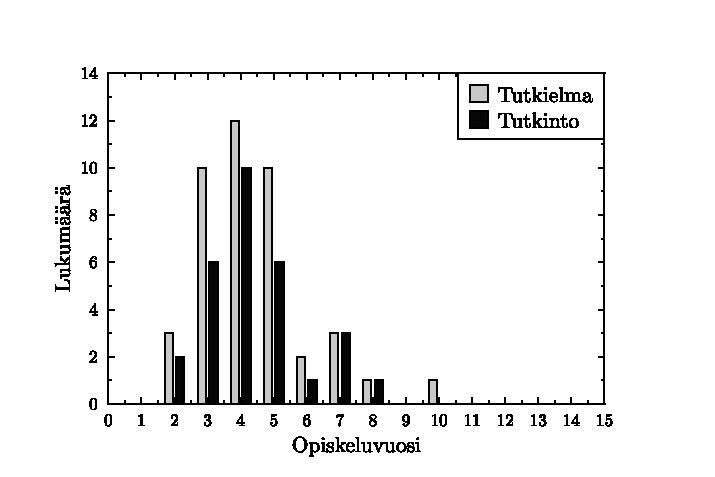
\includegraphics[width=\textwidth]{mallikuvio}
   \caption{Valmistuneiden kandidaatintutkielmien jakauma tekijän opiskeluvuoden mukaan Jyväskylän yliopiston fysiikan laitoksella 2014 ($n = 42$); tutkintojen jakauma opiskeluvuoden mukaan, kun tutkielma on valmistunut 2014 ($n = 29$; tilanne 4.3.2015). (Kuva: Jussi Maunuksela, 2015)}
   \label{fig:esim-kuvio}
\end{figure}

\section{Conclusions}
\label{sec:conclusions}

Loppuluvussa arvioidaan tutkimusta ja sen tuloksia. \lipsum[1]

\lipsum[2-3]

\nocite{*}

% --------------------------------------------------------------------------
% LÄHTEET
% --------------------------------------------------------------------------
\addcontentsline{toc}{section}{References}
\printbibliography

% --------------------------------------------------------------------------
% LIITTEET
% --------------------------------------------------------------------------
\appendix

\section{First appendix}
\label{sec:first-appendix}

\lipsum[2-3]

\section{Second appendix}
\label{sec:second-appendix}

\lipsum[2-3]

\end{document}

